\documentclass{article}
\newcommand*{\mv}[1]{\mathbf{#1}} % my vector
\newcommand*{\mm}[1]{\mathbf{#1}} % my matrix
\newcommand*{\norm}[1]{\lVert #1 \rVert} % euclidean norm

\usepackage[utf8]{inputenc}
\usepackage{graphicx}
\usepackage{amsmath, amssymb}
\usepackage[colorlinks=true,linkcolor=blue,citecolor=black]{hyperref}

\title{Safe Learning in Robotics}
\date{2025-07-21}
\author{}

\begin{document}

\maketitle

\tableofcontents

%%%%%%%%%%%%%%%%%%%%%%%%%%%%%%%%
% Chap Abstract
%%%%%%%%%%%%%%%%%%%%%%%%%%%%%%%%

\section*{Abstract}

This article provides a concise but holistic review of the recent advances made in using machine learning to achieve safe decision making under uncertainties, with a focus on unifying the language and frameworks used in control theory and reinforcement learning research.

%%%%%%%%%%%%%%%%%%%%%%%%%%%%%%%%
% Chap1 Introduction
%%%%%%%%%%%%%%%%%%%%%%%%%%%%%%%%

\section{Introduction}

Robotics researchers strive to design system taht can operate autonomously in increasingly complex scenarios, often in close proximity to humans.
Uncertainties arise from various sources.
For example, the robot dynamics may not be perfectly modeled, sensor measurements may be noisy, and/or the operating environment may not be well-characterized or may include other agents whose dynamics and plans are not known.
In recent years, the research community has multiplied its efforts to leverage data-based approaches to address this problem. (learning-based approach)
A crucial, domain-specific challenge of learning for robot control is not only for the optimized policy but also during training, to avoid costly hardware failures and improve convergence.
Both control theory and machine learning (reinforcement learning) have proposed approaches to tackle this problem.
\begin{itemize}
    \item Control theory has traditionally taken a model-driven approach: it leverages a given dynamics model and provides guarantees with respect to known operating conditions.
    \item RL has traditionally taken a data-driven approach, which makes it highly adaptable to new contexts at the expense of providing formal guarantees.
    \begin{itemize}
        \item RL, however, transfer to real systems remains a research area in itself.
    \end{itemize}
\end{itemize}
In this article, we provide a bird's eye view of the most recent work in learning-based control and reinforcement learning that implement safety and provide safety guarantees for robot control.
\begin{figure*}[h]
    \centering
    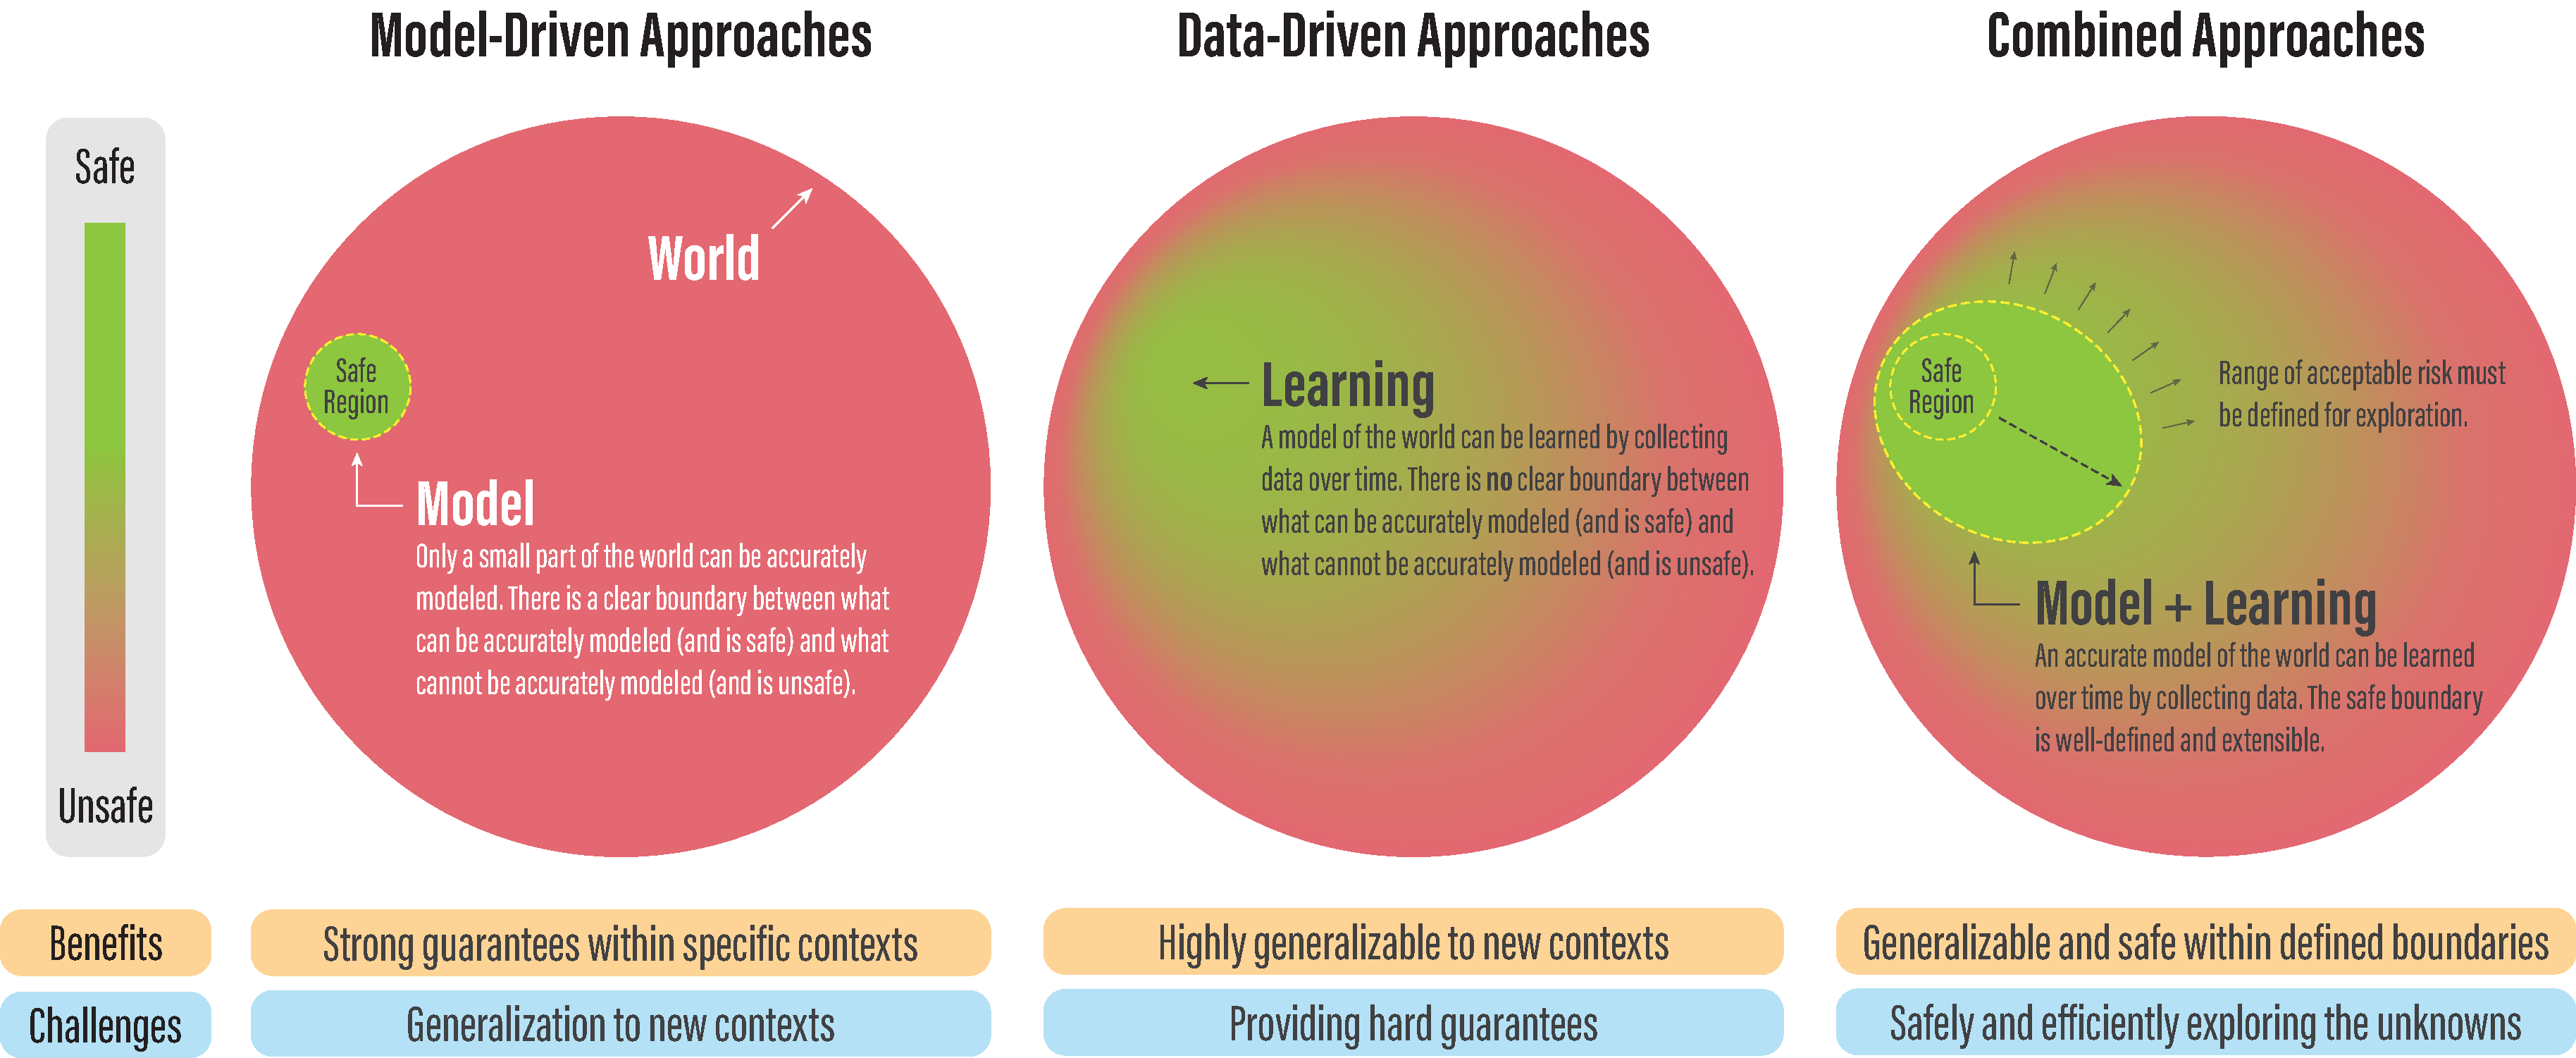
\includegraphics[width=1.0\textwidth]{imgs/problem_illustration.pdf}
    \caption{A comparison of model-driven, data-driven, and combined approaches.}
\end{figure*}

%%%%%%%%%%%%%%%%%%%%%%%%%%%%%%%%
% Chap2 Related Works
%%%%%%%%%%%%%%%%%%%%%%%%%%%%%%%%

\section{Preliminaries}

\subsection{Problem Statement}

We formulate the safe learning control problem as an optimization problem to capture the efforts of both the control and RL communities.
The optimization problem has three main components:
\begin{itemize}
    \item \textbf{System model} that describe the dynamic behavior of the robot.
    \item \textbf{Cost function} that defines the control objective or task goal.
    \item \textbf{Set of constraints} that specify the safety requirements.
\end{itemize}
The goal is to find a controller or policy that computes commands (also called inputs) that enable the system to fulfill the task while respecting given safety constraints.

\subsection{System Model}

We consider a robot whose dynamics can be represented by the following discrete-time model:
\begin{equation} \label{eq:system_model}
    \mv{x}_{k + 1} = \mv{f}_k(\mv{x}_k, \mv{u}_k, \mv{w}_k),
\end{equation}
where $\mv{k} \in \mathbb{Z}_{\geq 0}$ is the discrete-time index, $\mv{x}_k \in \mathbb{X}$ is the state with $\mathbb{X}$ denoting the state space.
$\mv{u}_k \in \mathbb{U}$ is the input with $\mathbb{U}$ denoting the input space, $\mv{f}_k$ is the dyanmics model of the robot, $\mv{w}_k \in \mathbb{W}$ is the process noise distributed according to a distribution $W$.
Throughout this review, we assume direct access to (possibly noisy) measurements of the robot state $\mv{x}_k$ and neglect the problem of state estimation.
The dynamics model in Eq. \eqref{eq:system_model} can be equivalently as a state transition probability function $T_k(\mv{x}_{k + 1}|\mv{x}_k, \mv{u}_k)$, commonly seen in RL approaches.

\subsection{Cost Function}

The robot's task is defined by a cost function.
We consider a finite-horizon optimal control problem with time horizon $N$.
Given an initial state $\mv{x}_0$, the cost function is computed based on the sequence of states $\mv{x}_{0:N} = \{\mv{x}_0, \mv{x}_1, \ldots, \mv{x}_N\}$ and the sequence of inputs $\mv{u}_{0:N-1} = \{\mv{u}_0, \mv{u}_1, \ldots, \mv{u}_{N-1}\}$:
\begin{equation}
    J(\mv{x}_{0:N}, \mv{u}_{0:N-1}) = l_N(\mv{x}_N) + \sum^{N - 1}_{k = 0} l_k(\mv{x}_k, \mv{u}_k),
\end{equation}
where $l_k : \mathbb{X} \times \mathbb{U} \mapsto \mathbb{R}$ is the stage cost incurred at each time step $k$, and $l_N: \mathbb{X} \mapsto \mathbb{R}$ is the terminal cost incurred at the end of $N$-step horizon.
The stage and terminal cost functions map the state and input sequences, which may be random variables, to a real number.
We formulate a cost minimization problem for safe learning control, while RL typically solves a reward maximization problem.

\subsection{Safety Constraints}

Safety constraints ensure, or encourage, the safe operation of the robot and include:
\begin{itemize}
    \item state constraints $\mathbb{X}_c \subseteq \mathbb{X}$, which defines the set of safe operating states
    \item input constraints $\mathbb{U}_c \subseteq \mathbb{U}$
    \item stability guarantees
    \begin{itemize}
        \item To encode the safety constraints, we define $n_c$ constraint functions: $\mv{c}_k(\mv{x}_k, \mv{u}_k, \mv{w}_k) \in \mathbb{R}^{n_c}$ with each constraint $c^j_k$ being a real-valued, time-varying function.
        \item We introduce three levels of safety: hard, probabilistic(chance), and soft.
    \end{itemize}
\end{itemize}

\subsubsection{Safety level 3: Constraint Satisfaction Guaranteed}
The system satisfies hard constraints:
\begin{equation} \label{eq:hard_constraint}
    c^j_k(\mv{x}_k, \mv{u}_k, \mv{w}_k) \leq 0
\end{equation}
for all times $k \in \{0, \ldots, N\}$ and constraint indexes $j \in \{1, \ldots, n_c\}$.

\subsubsection{Safety level 2: Constraint Satisfaction with Probability p}
The system satisfies probabilistic constraints:
\begin{equation} \label{eq:probabilistic_constraint}
    \Pr \left( c^j_k (\mv{x}_k, \mv{u}_k, \mv{w}_k) \leq 0 \right) \geq p^j
\end{equation}
where $\Pr(\cdot)$ denotes the probability and $p^j \in (0, 1)$ defines the likelihood of the $j$-th constraint being satisfied, with $j \in \{1, \ldots, n_c\}$ and for all times $k \in \{0, \ldots, N\}$.
The chance constraint in Eq. \eqref{eq:probabilistic_constraint} is identical to the hard constraint in Eq. \eqref{eq:hard_constraint} for $p^j = 1$.

\subsubsection{Safety Level 1: Constraint Satisfaction Encouraged}

The system encourages constraint satisfaction.
This can be achieved in different ways.
One way is to add a penalty term to the objective function that discourages the violation of constraints with a high cost.
A non-negative $\epsilon_j$ is added to the right-hand side of the inequality in Eq. \eqref{eq:hard_constraint}, for all times $k \in \{0, \ldots, N\}$ and constraint indexes $j \in \{1, \ldots, n_c\}$:
\begin{equation} \label{eq:soft_constraint}
    c^j_k(\mv{x}_k, \mv{u}_k, \mv{w}_k) \leq \epsilon_j
\end{equation}
and an appropriate penalty term $l_\epsilon(\epsilon) \geq 0$ with $l_\epsilon(\epsilon) = 0 \Longleftrightarrow \epsilon = 0$ is added to the objective function. (It means there is no penalty when the constraint is satisfied.)
The vector $\epsilon$ includes all elements $\epsilon_j$ and is an additional variable of the optimization problem.

\noindent Alternatively, although $c^j_k(\mv{x}_k, \mv{u}_k, \mv{w}_k)$ is a step-wise quantity, some approaches only aim to provide guarantees on its expected value $\mathbb{E}[\cdot]$ on a trajectory level:
\begin{equation} \label{eq:expected_constraint}
    J_{c^j} = \mathbb{E} \left[ \sum^{N - 1}_{k = 0} c^j_k(\mv{x}_k, \mv{u}_k, \mv{w}_k) \right] \leq d_j,
\end{equation}
where $J_{c^j}$ represents the expected total constraint cost, and $d_j$ defines the corresponding constraint threshold.
The constraint function can optionally be discounted as $\gamma^k c^j_k(\mv{x}_k, \mv{u}_k, \mv{w}_k)$ with the discount factor $\gamma \in [0, 1]$.

\begin{figure*}[h]
    \centering
    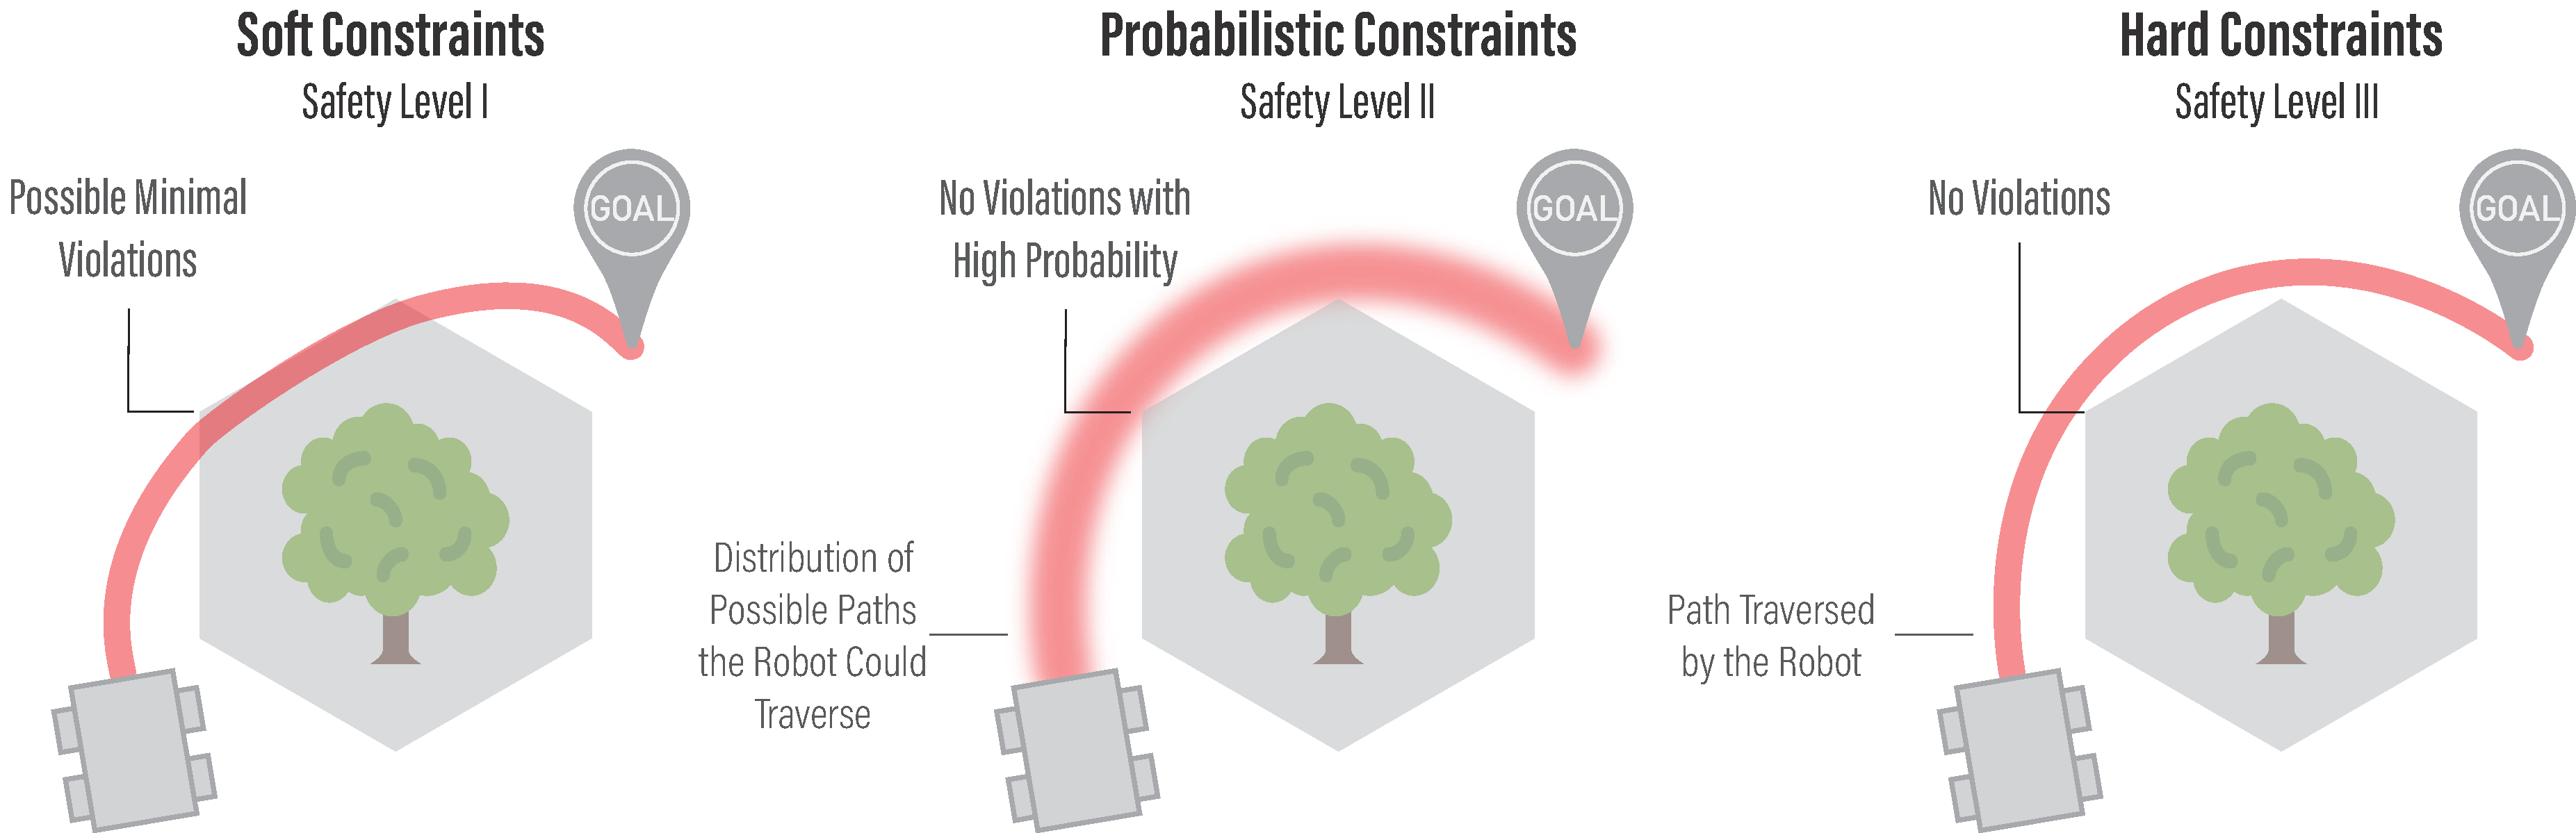
\includegraphics[width=1.0\textwidth]{imgs/safety_definition.pdf}
    \caption{Illustation of the different safety levels.}
\end{figure*}

\subsection{Formulation of the Safe Learning Control Problem}
The function introduced above, i.e., the system model $\mv{f}$, the constraints $\mv{c}$, and the cost function $J$, represent the true functions of the robot control problem.
In practice, $\mv{f}, \mv{c}$, and $J$ may be unknown or partially known.
Without loss of generality, we assume that each of the true functions $\mv{f}, \mv{c}$, and $J$ can be decomposed into a nominal component, $(\bar{\cdot})$, reflecting our prior knowledge, and an unknown component $(\hat{\cdot})$, to be learned from data.
For instance, the dynamics model $f$ can be decomposed as:
\begin{equation}
    \mv{f}_k(\mv{x}_k, \mv{u}_k, \mv{w}_k) = \bar{\mv{f}}_k(\mv{x}_k, \mv{u}_k) + \hat{\mv{f}}_k(\mv{x}_k, \mv{u}_k, \mv{w}_k),
\end{equation}
where $\bar{\mv{f}}$ is the prior dynamics mode and $\hat{\mv{f}}$ are the uncertain dynamics.
Safe learning control (SLC) leverages our prior knowledge $\mathcal{P} = \{\bar{\mv{f}}, \bar{\mv{c}}, \bar{J} \}$ and the data collected from the system $\mathcal{D} = \{\mv{x}^{(i)}, \mv{u}^{(i)}, \mv{c}^{(i)}, l^{(i)} \}^{i = \mathcal{D}}_{i = 0}$ to find a policy (or controller) $\pi_k(\mv{x}_k)$ that achieves the given task while respecting all safety constraints.
$(\cdot)^{(i)}$ denotes a sample  of a quantity $(\cdot)_k$ and $D$ is the data set size.
More specifically, we aim to find a policy $\pi_k$ that best approximates the true optimal policy $\pi^*_k$, which is the solution to the following optimization problem:
\begin{equation}
    \begin{aligned}
        J^{\pi^*}(\bar{\mv{x}}_0) 
        = \min_{\pi_{0:N -1}, \epsilon} &J(\mv{x}_{0:N}, \mv{u}_{0:N - 1}) + l_\epsilon(\epsilon) \\
        \text{s.t} \quad &\mv{x}_{k + 1}  = \mv{f}_k(\mv{x}_k, \mv{u}_k, \mv{w}_k), \quad \mv{w}_k \sim \mathcal{W}, \forall k \in \{0, \ldots, N - 1\}, \\
        & \mv{u}_k = \pi_k(\mv{x}_k),  \\
        & \mv{x}_0 = \bar{\mv{x}}_0, \\
        & \text{Safety constraints according to either} \\
        & \text{Eq. \eqref{eq:hard_constraint}, Eq. \eqref{eq:probabilistic_constraint}, Eq. \eqref{eq:soft_constraint} or Eq. \eqref{eq:expected_constraint}, and } \epsilon \geq 0, \\
    \end{aligned}
\end{equation}
where $\bar{\mv{x}}_0 \sim \mathcal{X}_0$ is the initial state with $\mathcal{X}_0$ being the initial state distribution, and $\epsilon$ and $l_\epsilon$ are introduced account for the soft safety constraint case (Eq. \eqref{eq:soft_constraint}) and are set to zero, for example, if only hard and probabilistic safety constraints are considered. (Eq. \eqref{eq:hard_constraint}, Eq. \eqref{eq:probabilistic_constraint})

\subsection{A Control Theory Perspective}

Typical assumptions are that a model of the system is available and it is either parameterized by an unknown parameter or it has bounded unknown dynamics and noise.

\subsubsection{Adaptive Control}

Adaptive control considers systems with parameteric uncertaintes and adapts the controller parameters online to optimize performance.
\footnote{
    A parameteric model depends on a finite number of parameters that may have a physical interpretation or reflect our prior knowledge about the system structure in other ways. 
    Parameteric uncertainty is the uncertainty in the model parameters.
}
Adaptive control requires knowledge of the parameteric form of the uncertainty and typically considers a dynamics model that t  hat is affine in $\mv{u}$ and the uncertain parameters $\mv{\theta \in \Theta}$:
\begin{equation}
    \mv{x}_{k + 1} = \bar{\mv{f}}_\mv{x}(\mv{x}_k) + \bar{\mv{f}}_\mv{u}(\mv{x}_k) \mv{u}_k + \bar{\mv{f}}_\theta(\mv{x}_k) \theta,
\end{equation}
where $\bar{\mv{f}}_\mv{x}, \bar{\mv{f}}_\mv{u}$, and $\bar{\mv{f}}_\theta$ are known functions often derived from first principles and $\Theta$ is a possibly bounded parameter set.
The control input is $\mv{u}_k = \pi(\mv{x}_k, \hat{\theta}_k)$, which is parameterized by $\hat{\theta}_k$.
\begin{itemize}
    \item The parameter $\hat{\theta}_k$ is adapted by using either a Lyapunov function to gurantee that the closed-loop system \footnote{A general system is given by $\mv{x}_{k + 1} = \mv{f}(\mv{x}_k, \mv{u}_k)$. If the input is given based on the state, i.e., $\mv{u}_k = \pi(\mv{x}_k)$, then the system is called a closed-loop system.} is stable.
    \item Model Reference Adaptive Control (MRAC) to make the system behave as a predefined stable reference model.
\end{itemize}
Adaptive control is typically limited to parameteric uncertainties and relies on a specific model structure.
Moreover, adaptive control approaches tend to "overfit" to the latest observations and convergence to the true parameters is generally not guranteed.
These limitations motivate the learning-based adaptive control approaches in Sec. % TODO: Add Sec. reference.

\subsubsection{Robust Control}

In contrast to adaptive control, which adapts to the parameters currently present, robust control finds a suitable controller for all possible disturbances, which can include unknown dynamics and noise, and keeps the controller unchanged after the initial design.
Robust control is largely limited to linear, time-invariant (LTI) systems with linear nominal model $\bar{\mv{f}}(\mv{x}_k, \mv{u}_k) = \bar{\mv{A}} \mv{x}_k + \bar{\mv{B}} \mv{u}_k$ and unknown dynamics $\hat{\mv{f}}_k(\mv{x}_k, \mv{u}_k, \mv{w}_k) = \hat{\mv{A}} \mv{x}_k + \hat{\mv{B}} \mv{u}_k + \mv{w}_k \in \mathbb{D}$, with $\mathbb{D}$ being known and bounded, and $\bar{\mv{A}}, \bar{\mv{B}}, \hat{\mv{A}}, \hat{\mv{B}}$ being static matrices of appropriate size.
That is,
\begin{equation}
    \mv{x}_{k + 1} =(\bar{\mv{A}} + \hat{\mv{A}}) \mv{x}_k + (\bar{\mv{B}} + \hat{\mv{B}}) \mv{u}_k + \mv{w}_k.
\end{equation}
Robust control design techniques yield controllers that are robustly stable for all $\hat{\mv{f}}_k \in \mathbb{D}$.
Robust control can be extended to nonlinear system whose dynamics can be decomposed into a linear nominal model $\bar{\mv{f}}$ and a nonlinear function $\hat{\mv{f}}$ with known bound $\hat{\mv{f}} \in \mathbb{D}$. \footnote{Do not confuse $\mathcal{D}$, which denotes the dataset collected from the system, with $\mathbb{D}$, which represents the disturbances set. }

\subsubsection{Robust Model Predictive Control (MPC)}


%%%%%%%%%%%%%%%%%%%%%%%%%%%%%%%%
% Chap3 Method
%%%%%%%%%%%%%%%%%%%%%%%%%%%%%%%%

\section{Method}

% Method description

%%%%%%%%%%%%%%%%%%%%%%%%%%%%%%%%
% Chap4 Experiment
%%%%%%%%%%%%%%%%%%%%%%%%%%%%%%%%

\section{Experiment}

% Experiment setup/results

%%%%%%%%%%%%%%%%%%%%%%%%%%%%%%%%
% Chap5 Discussion
%%%%%%%%%%%%%%%%%%%%%%%%%%%%%%%%

\section{Discussion}

% Discussion points

%%%%%%%%%%%%%%%%%%%%%%%%%%%%%%%%
% Chap6 Conclusion
%%%%%%%%%%%%%%%%%%%%%%%%%%%%%%%%

\section{Conclusion}

% Final conclusion

\end{document}
